\begin{figure}[htbp]
  \centering
  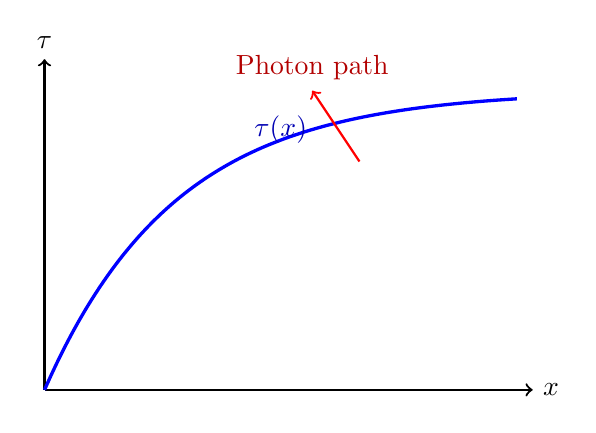
\begin{tikzpicture}
    % Axes
    \draw[->,thick] (0,0) -- (6.2,0) node[right] {$x$};
    \draw[->,thick] (0,0) -- (0,4.2) node[above] {$\tau$};
    % Clock-field profile  τ(x) = τ∞(1 − e^{-kx})
    \draw[very thick,blue,smooth,domain=0:6,samples=70]
         plot(\x,{3.8*(1-exp(-0.6*\x))});
    \node[blue!70!black] at (3,3.3) {$\tau(x)$};
    % Photon path arrow
    \draw[->,red,thick] (4,2.9) -- ++(-0.6,0.9)
         node[above,red!70!black]{Photon path};
  \end{tikzpicture}
  %-------------------------------------------------------------
  \caption{Illustrative gradient of the clock field $\tau$ along a photon trajectory.}
  \label{fig:ClockGradient}
\end{figure}
